% !TeX root = main.tex
%\newpage
%\setcounter{page}{1}
\section{Introduction}
\label{s:intro}

  Modern science and business involve using large amounts of data to perform various computational or learning tasks. The data required by a
particular research group or enterprise usually contain \textit{errors and inaccuracies} because of the following reasons:
\begin{CompactEnumerate}
  \item[-] the validity of the data changes dynamically. For example data involving home locations of customers or employees are
           not constant over time. Hence a set of data collected in a particular time frame probably is not going to remain valid for the
           future,
  \item[-] the data might be provided by other entities or collected online from a source that has no certification for their validity. For
           example data collected from crowdsourcing environments.
\end{CompactEnumerate}

\noindent We call a set of data with the property that only a subset of them is valid an \textit{unreliable data set}. The goal of this paper
is to develop theoretically established methods that lead to \textit{certified computation} over such data sets. Towards this goal we
assume that we have the  ability to \textit{verify} the validity of a record in our data set. Usually this verification process is costly and hence
it doesn't make sense to verify all the records in our data set every time we want to compute a function on them. On the other hand if the
majority or the most important part of the data are invalid then trying to find a valid subset could lead to essentially verifying the entire data set. In our work we introduce the concept of \textit{learning with certification}, in which we can distinguish between the following scenarios
\begin{CompactEnumerate}
  \item the value of the function that we computed on the unreliable data set is close to the value of the function computed on the valid
           subset of our data set,
  \item there exists at least one invalid record that could dramatically charge the value of the function that we want to compute.
\end{CompactEnumerate}
by verifying only a small number of records.
\smallskip

\noindent \textbf{Computations in Crowdsourcing.} Crowdsourcing \cite{DoanRH2011} is a popular instantiation of an unreliable data set,
where records are provided by a very large number of workers. These workers may need to put significant effort to extract high quality data
and without the right incentives they might choose not to do so giving, as a result, very noisy and unreliable reports. Experimental evidence
\cite{KazaiKKM2011, VuurensVE2011, WaisLCFGLMS2010} suggests that There are a large number of examples where crowdsourcing fails in practice
because of the unreliability of the data that it produces. An anecdotal failure of crowdsourcing is the example of Walmart's mechanism that
made the famous rapper Pitbull travel to the remote island of Kodiak, Alaska, see e.g., \cite{Pitbull12}. In 2012, Walmart asked their
customers to vote, through Facebook, their favorite local store. The store with the most votes would host a promotional performance by Pitbull.
Probably as a mean joke, a handful of people organized an \#ExilePitbull campaign, inviting Facebook users to vote for the most remote Walmart
store, at Kodiak. The campaign went viral and Pitbull performed at Kodiak, in July 2012. While the objective of Walmart was to learn the
location that would maximize attendance to the concert, the resulting outcome was terribly off because the incentives of the workers were
misaligned.

  Our work is motivated by these observations and aims through the use of verification to provide a generic approach that
guarantees high quality learning outcomes. Verification can be implemented either directly, in tasks such as peer grading,
by having an expert regrade the assignment, or indirectly, e.g. in the Walmart example by verifying the locations of the
voters. The main challenge in our framework it to minimize such verifications since they can be very costly.

\subsection{Our Model and Results}

  A data set is a set of records $\Workers$. The set $\Workers$ may contain, apart from the valid subset of records $\Truth$, a set of records
$\Workers \setminus \Truth$ that are invalid due to reasons that we described earlier. But how much does the presence of these invalid records
affect the output of the computation? The answer to this question depends on the number but also on the \textit{importance} of the invalid
records, where the importance depends on the specific computation task that we want to run.
%
%\begin{figure}[!h] \label{fig:crowdsourcing task}
%  \centering
%  {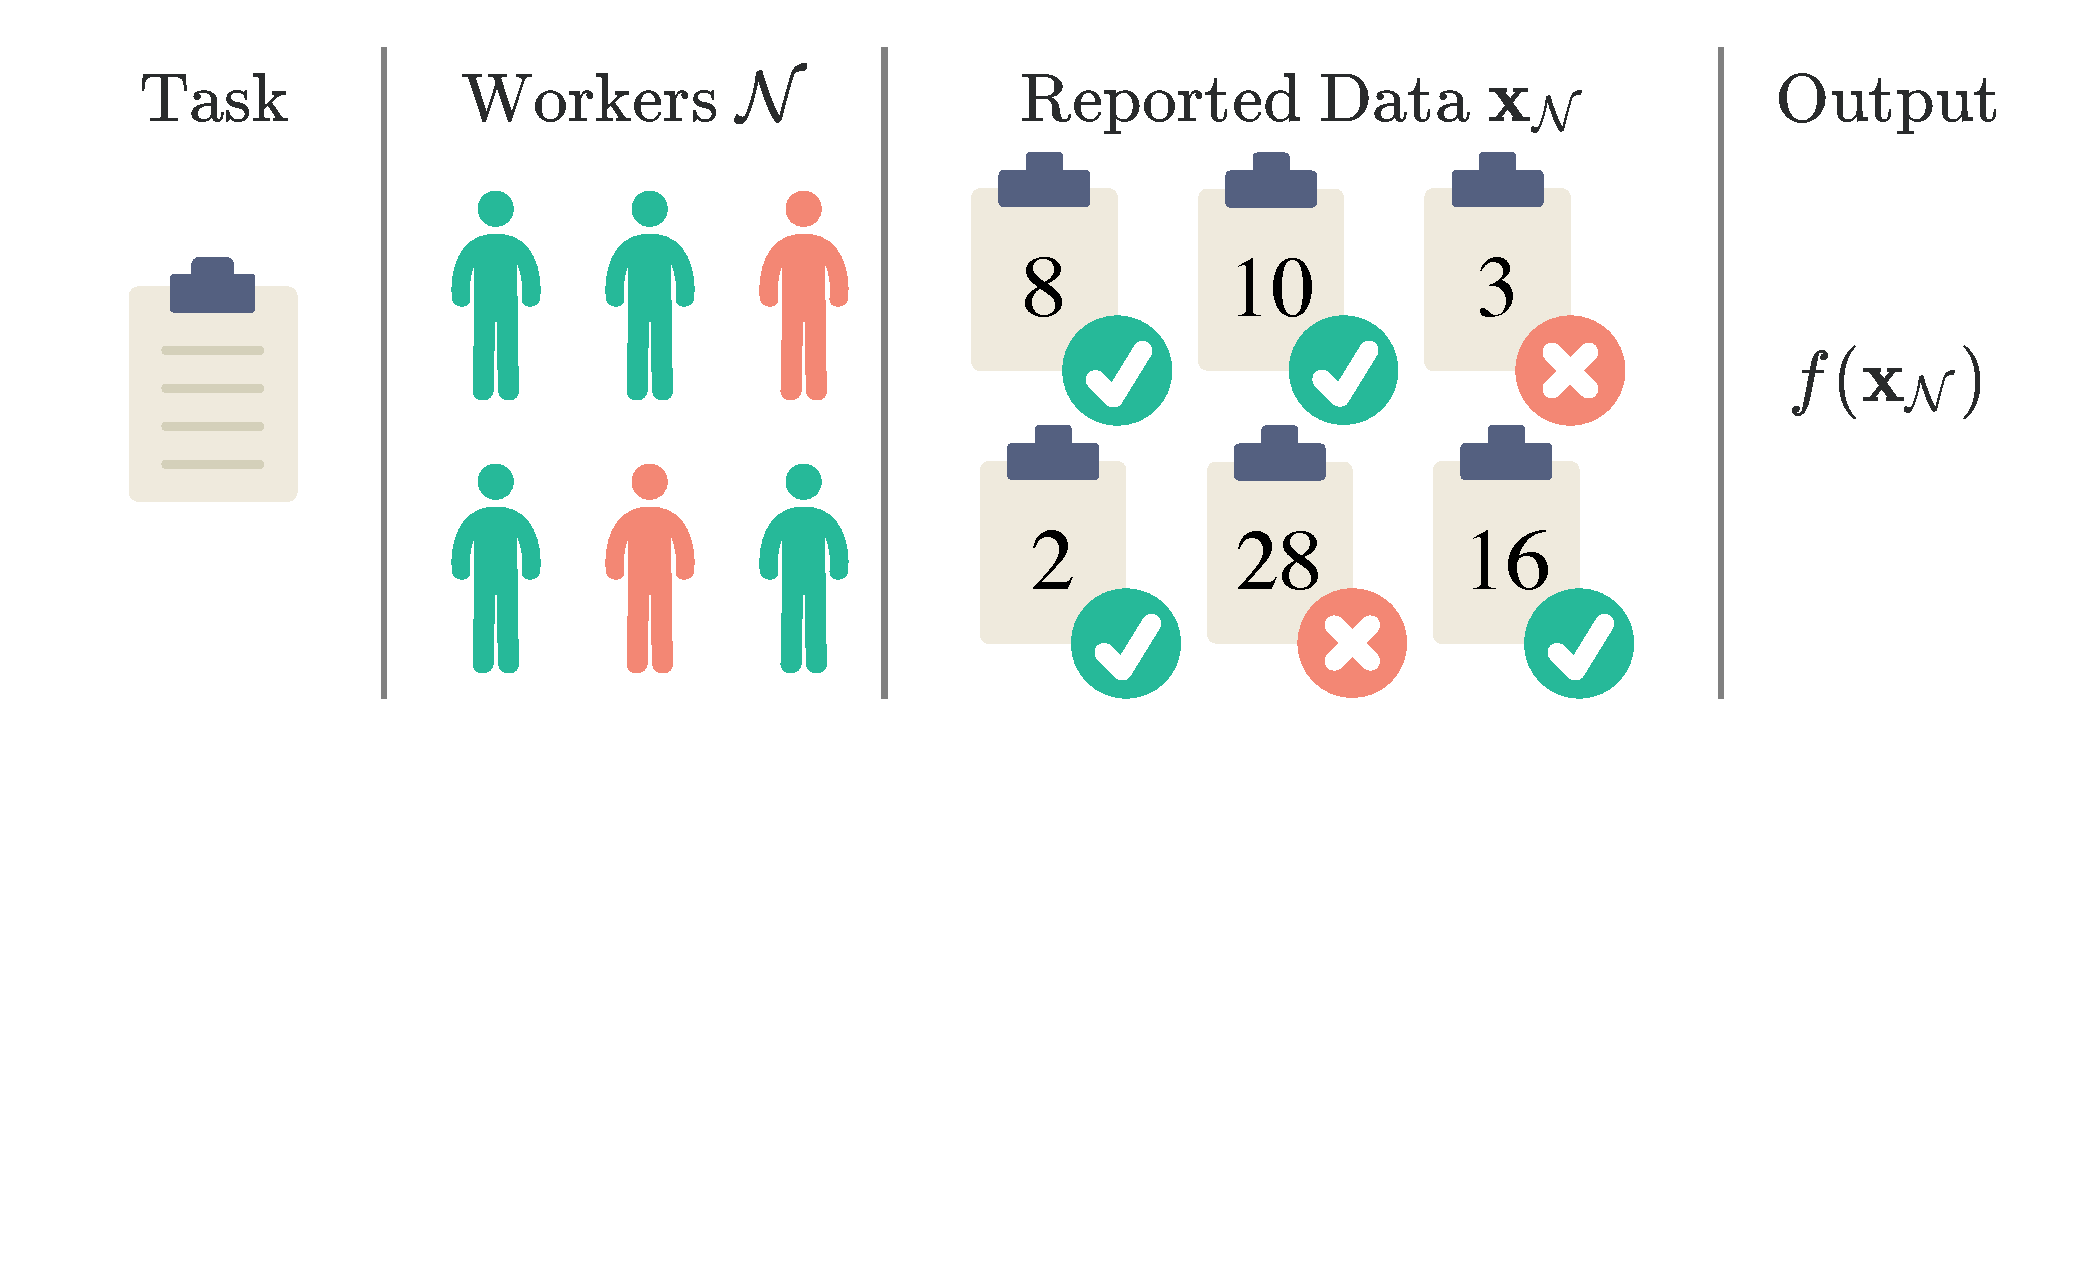
\includegraphics[clip, trim=2cm 9.5cm 1cm 1cm,width=0.65\textwidth]{figure1.pdf}}
%  \caption{A computation $f$ crowdsourced to a set of workers $\Workers$.}
%\end{figure}

  In order to assess whether the computed output is accurate, we can verify the validity of some of the records. Our goal is to verify as few
reports as possible and eventually be confident that the output of the computation is accurate. At this point we have to define a measure to
evaluate the accuracy of an output. Ideally, an accurate output is the output that we would get if all the records were valid. Such a benchmark,
however, is impossible to achieve as the correct values of the invalid records are unobservable. We instead focus on a simpler benchmark. We want
to decide whether given an unreliable data set the output of the computation based on $\Workers$ is close to the output of the computation based
only on $\Truth$. That is, if we could see which records are invalid and perform the computation task after discarding them, would the output
of the computation be close to the current value?

\paragraph{Certification Schemes} A positive answer to the question above is called \textit{certification} of the computation task based on the
unreliable data set $\Workers$. A negative answer is a witness that at least one record in $\Workers$ is invalid. Our first goal of this paper is to provide certification schemes for general computation
tasks that verify only a small number of records and can distinguish between these two cases.

\begin{figure}[!h] \label{fig:immunity}
  \centering
  {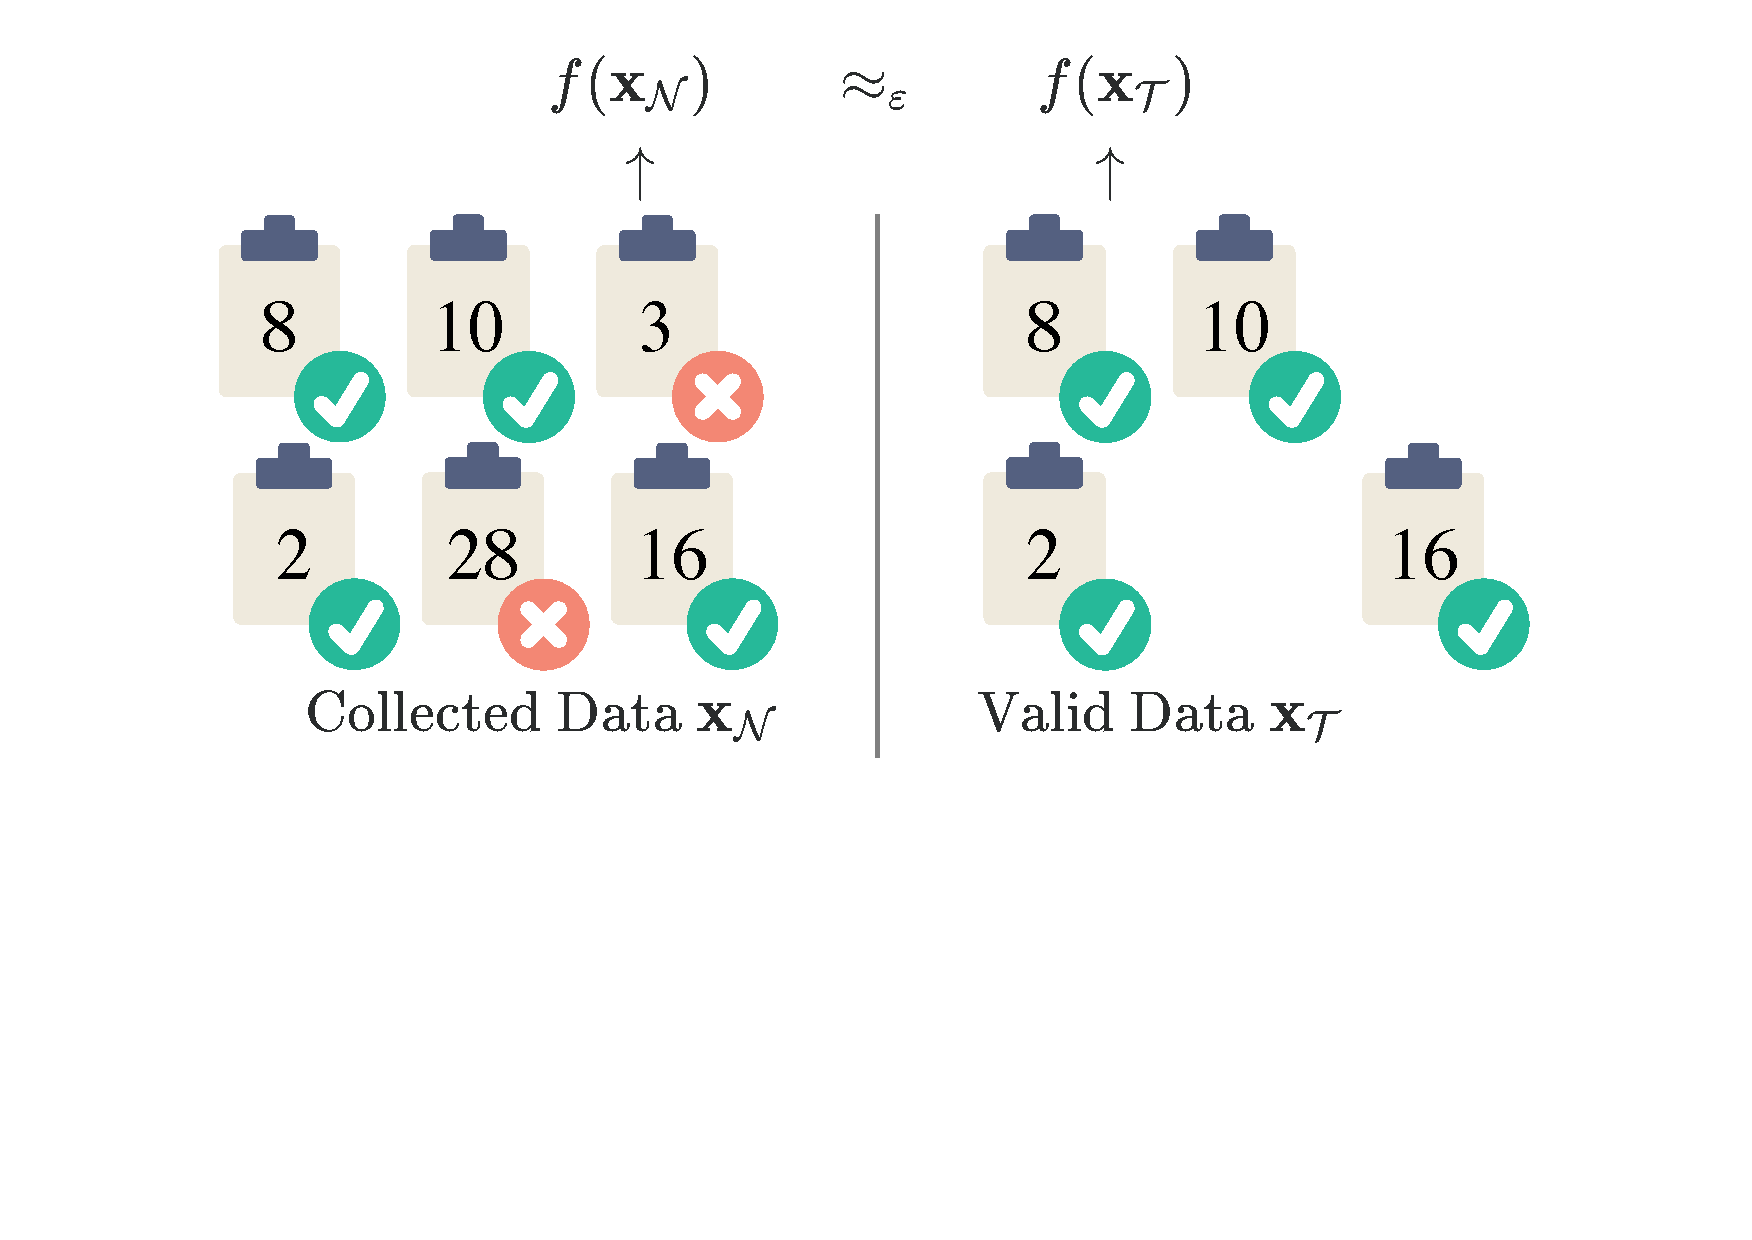
\includegraphics[clip, trim=2cm 8cm 2cm 1cm,width=0.45\textwidth]{figure2_new.pdf}}
  \caption{The property that a certification scheme certifies.}
\end{figure}

As a toy example of these models let us consider the simple function $f(\xw) = \max_{i \in \Workers} x_i$, where we assume that each record is a
real number $x_i \in \reals$. For the certification task we want to check whether $f(\xw) = f(\xt)$ or not. This can be easily done by checking
whether the record $i^* = \arg \max_{i \in \Workers} x_i$ is valid or not.

Not all functions though have such efficient deterministic and exact correction schemes. For several functions, we can obtain randomized
certification schemes that succeed with high probability and certify that the output is close up to a multiplicative factor. Moreover, for some
functions it might not even be possible to efficiently certify them without certifying almost everything. One extreme such example is a threshold
function that is 1 if all records are valid and 0 otherwise, $\mathbb{I}_{\Workers=\Truth}$ where we cannot obtain any meaningful approximation
without verifying $\Omega(n)$ records of $\Workers$.

In Section~\ref{sec:certification}, we provide efficient certification schemes for many different functions. Our results are the following:
\begin{Itemize}
  \item[-] {\bf sum function.} We start by presenting a randomized scheme for certifying the sum of all records that uses only
           $O(\frac 1 \varepsilon)$ verifications to certify correctness up to a multiplicative factor $1 \pm \varepsilon$. This is a very useful
           primitive that can be used in several different tasks: For example for computing the average, we can compute and certify the total sum
           of records and divide by the total number of records which we can also certify as another summation task. Another example is the
           \emph{max-of-sums} function, where as in the Walmart example we presented earlier, agents vote on different categories and the goal is
           to compute the total category that has the maximum number (or sum) of valid records. This can be easily certified by computing the max
           of all sums of records and certifying that this sum is approximately correct.
  \item[-] {\bf functions given by linear programs.} We then study the set of functions  expressible as LPs where the input data
           corresponds to either variables or constraints of the LP. We show that for functions expressible as packing or covering LPs, only
           $O(\frac 1 \varepsilon)$ verifications to certify correctness up to a multiplicative factor $1 \pm \varepsilon$ while for more general
           LPs we provide a deterministic scheme that depends on the dimensionality (number of variables or constraints).
  \item[-] {\bf instance-optimal schemes.} To study more general functions, we devise a linear program that characterizes (up to a constant factor)
           for any given instance the minimum number of verifications needed for approximate certification. We show that even though optimal
           certification schemes may be arbitrarily complex, there are simple schemes that verify records independently that are almost-optimal.
  \item[-] {\bf Main theorem for certification.} Our main most general result is that we can provide explicit solutions to the instance optimal
           linear program for a large class of different objectives that satisfy a $w$-Lipschitz property. We illustrate the flexibility of this
           constraint by showing that even very complex functions that correspond to NP-hard problems satisfy the $w$-Lipschitz property.
           Specifically, using our general theorem, we prove this for the TSP problem and the Steiner tree problems where we show that the
           certification complexity is only $O(\frac 1 \varepsilon)$. These capture settings where agents report their locations in a metric space
           and the goal is to design an optimal tour that visits all of them (TSP) or connecting them in a network by minimizing total cost
           (Steiner tree).
\end{Itemize}

\paragraph{Correction Schemes} Although very useful, the certification process fails when at least one invalid record is found. Naturally the next
question to ask is how we can proceed in order to actually compute the value of the function that we are interested in by throwing away the invalid
records. In a worst case example where all records are invalid, we would need to verify all the agents to complete the correction task. To get a more
meaningful and realistic measure of the verification complexity of a correction task, we carefully define it in terms of a budget $B$. For verification
complexity $V$, we assume that the designer has an initial budget for verifications $B = V$ which decreases as he performs verifications but might
increase every time he finds an invalid record.
The rationale behind the increase is that  verifications of incorrect records lead to their removal from the data set, which makes it more accurate. Therefore, in this model we measure the number of verifications needed to correct one incorrect record.
 %The rationale behind the increase is that often times verifications of incorrect records may be a lot
%less costly or the might be associated with penalties which make up for the cost of additional verifications.
We distinguish correction schemes
into two models depending on the budget increase.

In the \textit{weak correction} model, the budget increases by $V$ every time an invalid record is found. This means that finding an invalid record allows
us to restart the process from the beginning.

In the \textit{strong correction} model, the budget does not increase but does not decrease either. This means that verification of invalid records is
costless.

Of course, as we said, in the worst case a correction scheme has to verify all the data in the data set which is not realistic. However,  during the correction procedure for specific tasks it would be reasonable to have an upper bound on the number of invalid data that we are willing to verify before dismissing the entire data set for being too corrupted.
In particular, if the correction scheme
succeeds within the verification budgets we have an accurate output to our computation task. Otherwise, we can conclude that our data set is too corrupted and hence we need to collect the data from the beginning.
%
%\begin{figure}[!h]
%  \centering
%t   {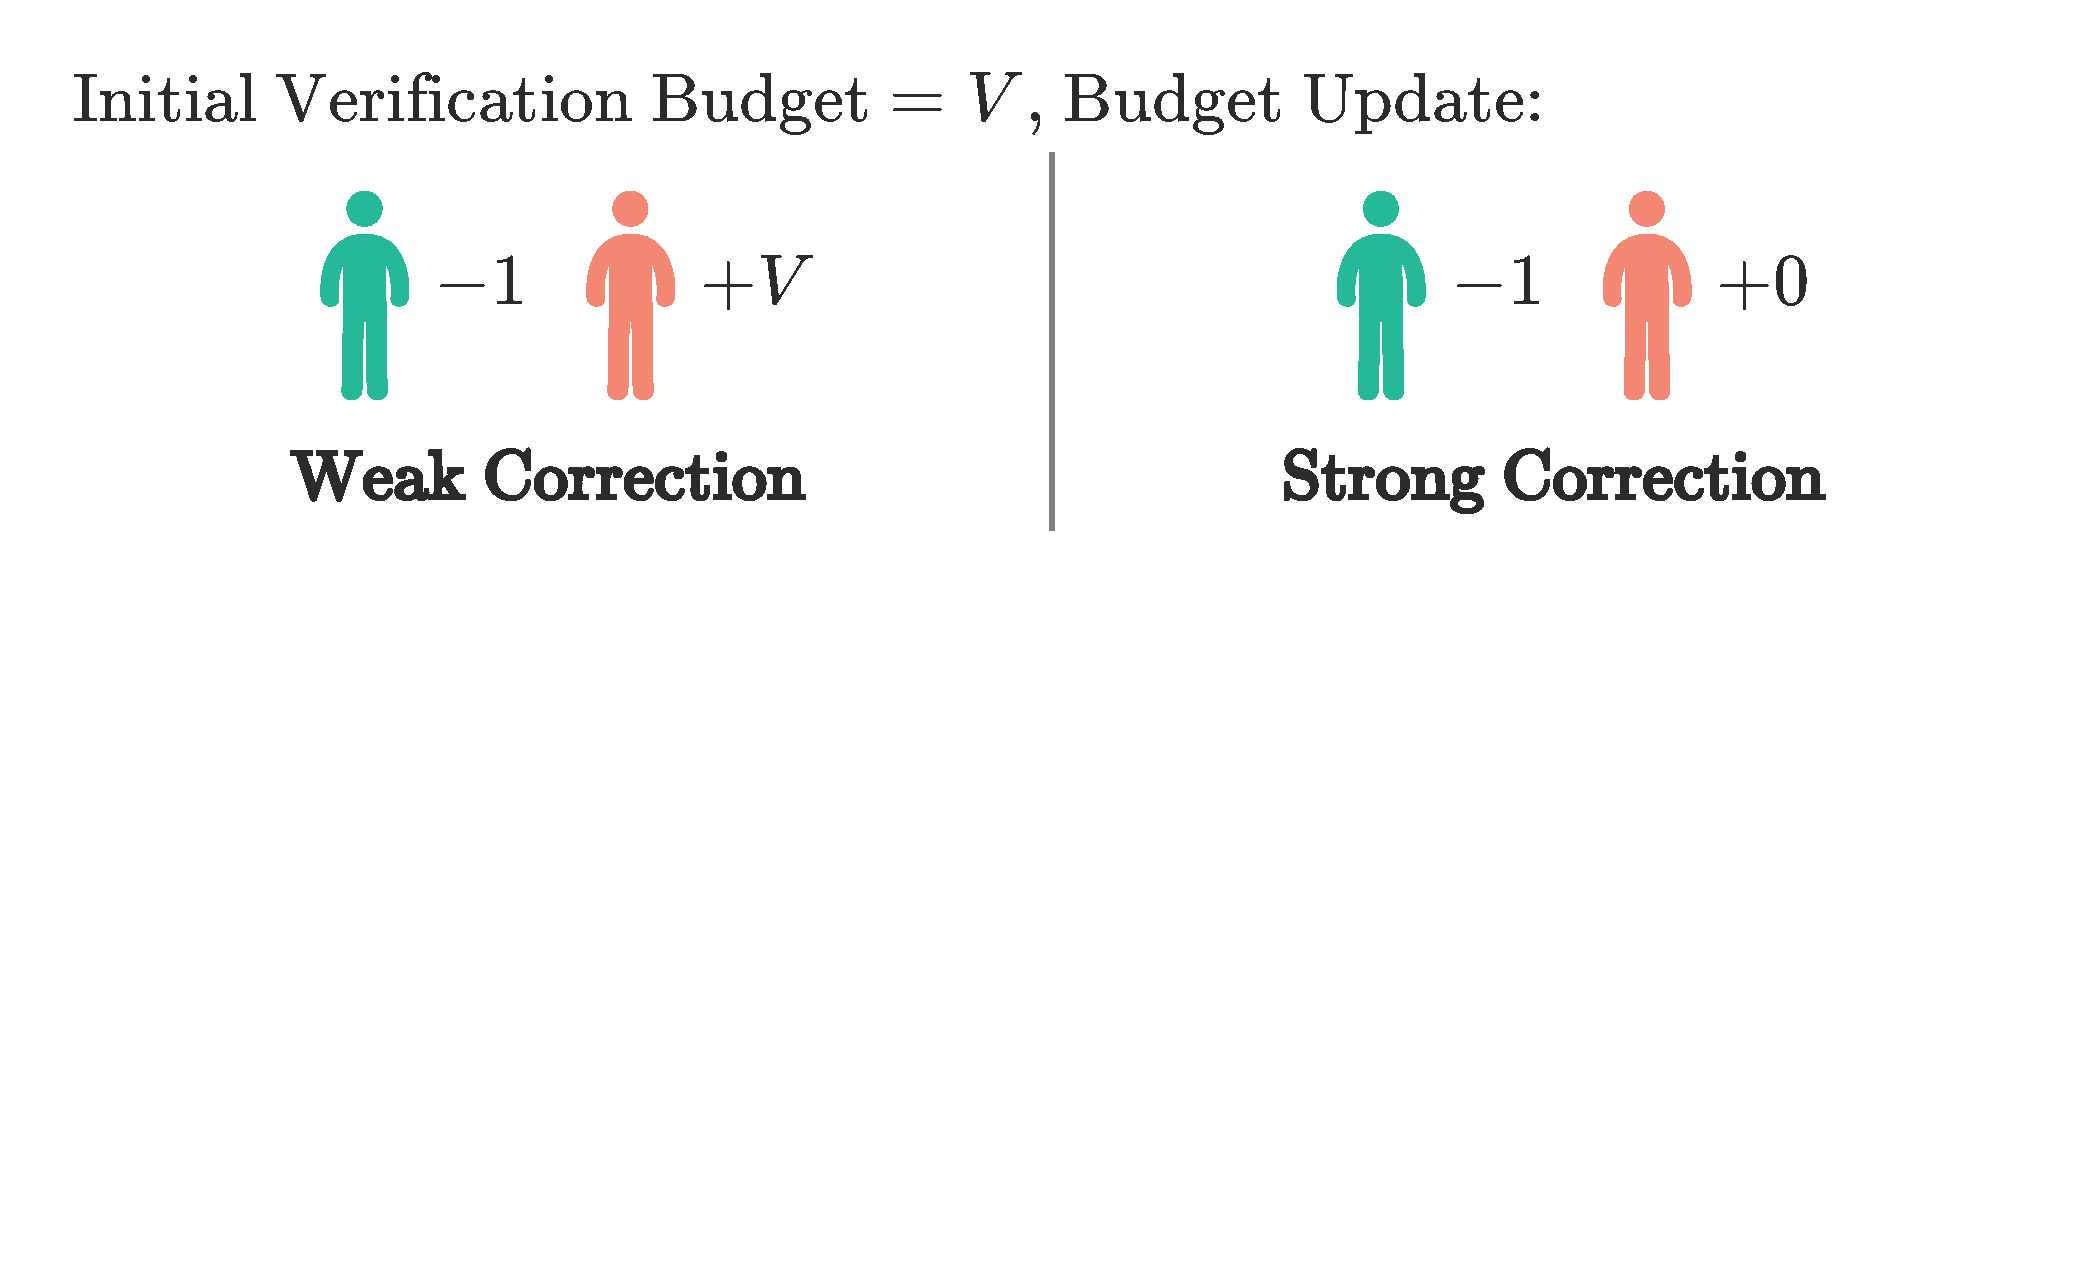
\includegraphics[clip, trim=1cm 12.5cm 2cm 1cm,width=0.6\textwidth]{figure3.pdf}}
%  \caption{The comparison of weak and strong correction in terms of verification budget.}
%\label{fig:budget}
%\end{figure}

  Notice that in the example of the $\max$ function, if the certification fails then we can continue by checking the second largest record and so on
until we find a valid record which will give us the value $f(\xt)$ precisely. %This last scheme it is easy to see that it is both a weak and strong
%correction scheme.
However, strong correction schemes are much harder to obtain than weak ones in general.

  If our computation or learning task has a deterministic certification scheme, e.g. the $\max$ function, it is easy to obtain weak correction
schemes by repeating the certification scheme until success. For randomized schemes though, one needs to be more careful as it is possible that errors
can accumulate. This is easy to fix by requiring that the certification scheme fails with probability at most $1/n$. However, this increases the total
weak-verification complexity by a logarithmic factor.

  In Section~\ref{sec:wcorr}, we prove our main result for weak correction schemes which implies that such an increase is not necessary and it is
possible to obtain weak correction schemes with the same complexity as the underlying certification scheme (up to constant factors). To do this, we run
the certification scheme many times and do not stop the first time it succeeds but continue until the total number of successes is more than the number
of failures. A random walk argument guarantees that this produces the correct answer with constant probability. If the objective function is not
monotone, additional care is needed to get the same guarantee.

  While weak correction schemes with good verification complexity exist for all tasks that we can efficiently certify, strong correction schemes are
more rare. In Section~\ref{sec:scorr}, we show that it is possible to obtain strong correction schemes for the sum function using only
$O(\frac 1 {\varepsilon^2})$ verifications of valid records. Since that many verifications are necessary to get a $1 \pm \varepsilon$ multiplicative
approximation for the sum, this implies a gap between the weak and strong correction models. The gap between them can be arbitrarily large though. As an example, the max-of-sums function we discussed earlier has certification and weak-correction complexity $O(\frac 1 {\varepsilon})$, although it is impossible to get a constant factor approximation in the strong correction model without verifying $\Omega(n)$ valid records.

  Despite the impossibility of obtaining strong correction schemes even for simple functions such as the max-of-sums, we can show that efficient
certification schemes exist for quite general optimization objectives. We prove (Theorem~\ref{thm:sCorrection}) a very interesting and tight connection
of strong correction schemes with \textit{sublinear algorithms that use conditional sampling}~\cite{GouleakisTZ2017}. We can exploit this connection to
directly obtain efficient strong correction schemes. This gives efficient schemes for general optimization tasks such as clustering, minimum spanning tree,
TSP and Steiner tree that capture settings where agent reports lie on some metric space.

\begin{comment}
\paragraph{Designing Incentive Compatible Mechanisms.} Our work presents a generic framework for designing schemes to verify the output of a computation
based on noisy and possibly adversarial reports from strategic agents. We can view each report as a record in an unreliable data set that is valid if the
corresponding report is truthful and invalid otherwise. Our work does not attempt to model incentives directly but aims to do the best possible given the
reported data. Coupled with a scheme that rewards agents according to their contribution to the objective (e.g. based on Shapley values), it can yield
approximately group-strategy proof mechanisms. This is because, any group of agents that has significant contribution to the objective and deviates will
be verified and excluded. In addition, even though in the worst-case correction schemes may need to verify everyone, the number of false reports is not
expected to be very large if agents know that they cannot affect the outcome by misreporting. 
\end{comment}

\subsection{Related Work}
Our certification task resembles the task of property testing, as formalized in \cite{GGR96},
where one has to decide whether the data has a particular property versus being $\varepsilon$-far from it in some distance metric. In our case, the property we want to test is whether the evaluation of the function on all the collected data is equal to its evaluation on the subset of the valid data only.

  Our correction task is related to a large body of work in statistics on how to
deal with noisy or incomplete datasets. Several methods have been proposed for dealing with missing data. The popular method of imputation
\cite{Rubin:87,book:imputation,book:incomplete:data} corrects the dataset by filling in the missing values using the
maximum likelihood estimates.

In addition, the field of robust statistics \cite{hampel80, huber11} deals with the problem of designing estimators when the dataset contains random or adversarially corrupted datapoints. Several efficient algorithmic results have recently appeared in the context of robust parameter estimation and distribution learning \cite{DKK+16,DKK+17,DKK+18,DKS17,LRV16}. The goal of these works is to learn the parameters of a multidimensional distribution, that belongs to a known parametric family, while a constant fraction of the samples have been adversarially corrupted.
\cite{CharikarSG17} deal with parameter estimation in cases where more than half of the dataset is corrupted and identification is impossible by providing a list of candidate estimates. They show that the correct estimate can be chosen as long as a small ``verified'' set of data is provided. In contrast to \cite{CharikarSG17}, the verification oracle in our model allows us to verify any subset of datapoints but verification is costly.   
\cite{SVC16} consider similar verification access to the dataset in crowdsourced peer grading settings.

Selective verification of datapoints has also been explored in the context of mechanism design. \cite{FotakisTZ16} study mechanisms with verification and achieve truthfulness by solving a task similar to certification in social choice problems.

Finally, another related branch of literature considers the task of correcting datasets through local queries (\cite{JhaR11,BlumLR90,BhattacharyyaGJJRW12,SacksS10,AilonCCSL08,CanonneGR16}). For example, using local queries, \cite{AilonCCSL08} correct datasets to ensure monotonicity and other structural properties. \cite{CanonneGR16} solve similar local correction tasks for noisy probability distributions. 


